For the numerical experiments, we firstly run the same experiments of \cite{buzna2007efficient} anc reproduce \emph{figure 2} in original paper\cite{buzna2007efficient}. Then we compare the strategy derivated by our optimization with these six heuristic strategies.

\subsection{Reproducing Experiments of Original Paper}

In order to prove the correctness of our model and codes, we firstly run the same experiments in original paper\cite{buzna2007efficient} and reproduce the \emph{figure 2} in \cite{buzna2007efficient}.


\begin{figure}	
	\centering
	\begin{subfigure}[t]{0.8\textwidth}
		\centering
		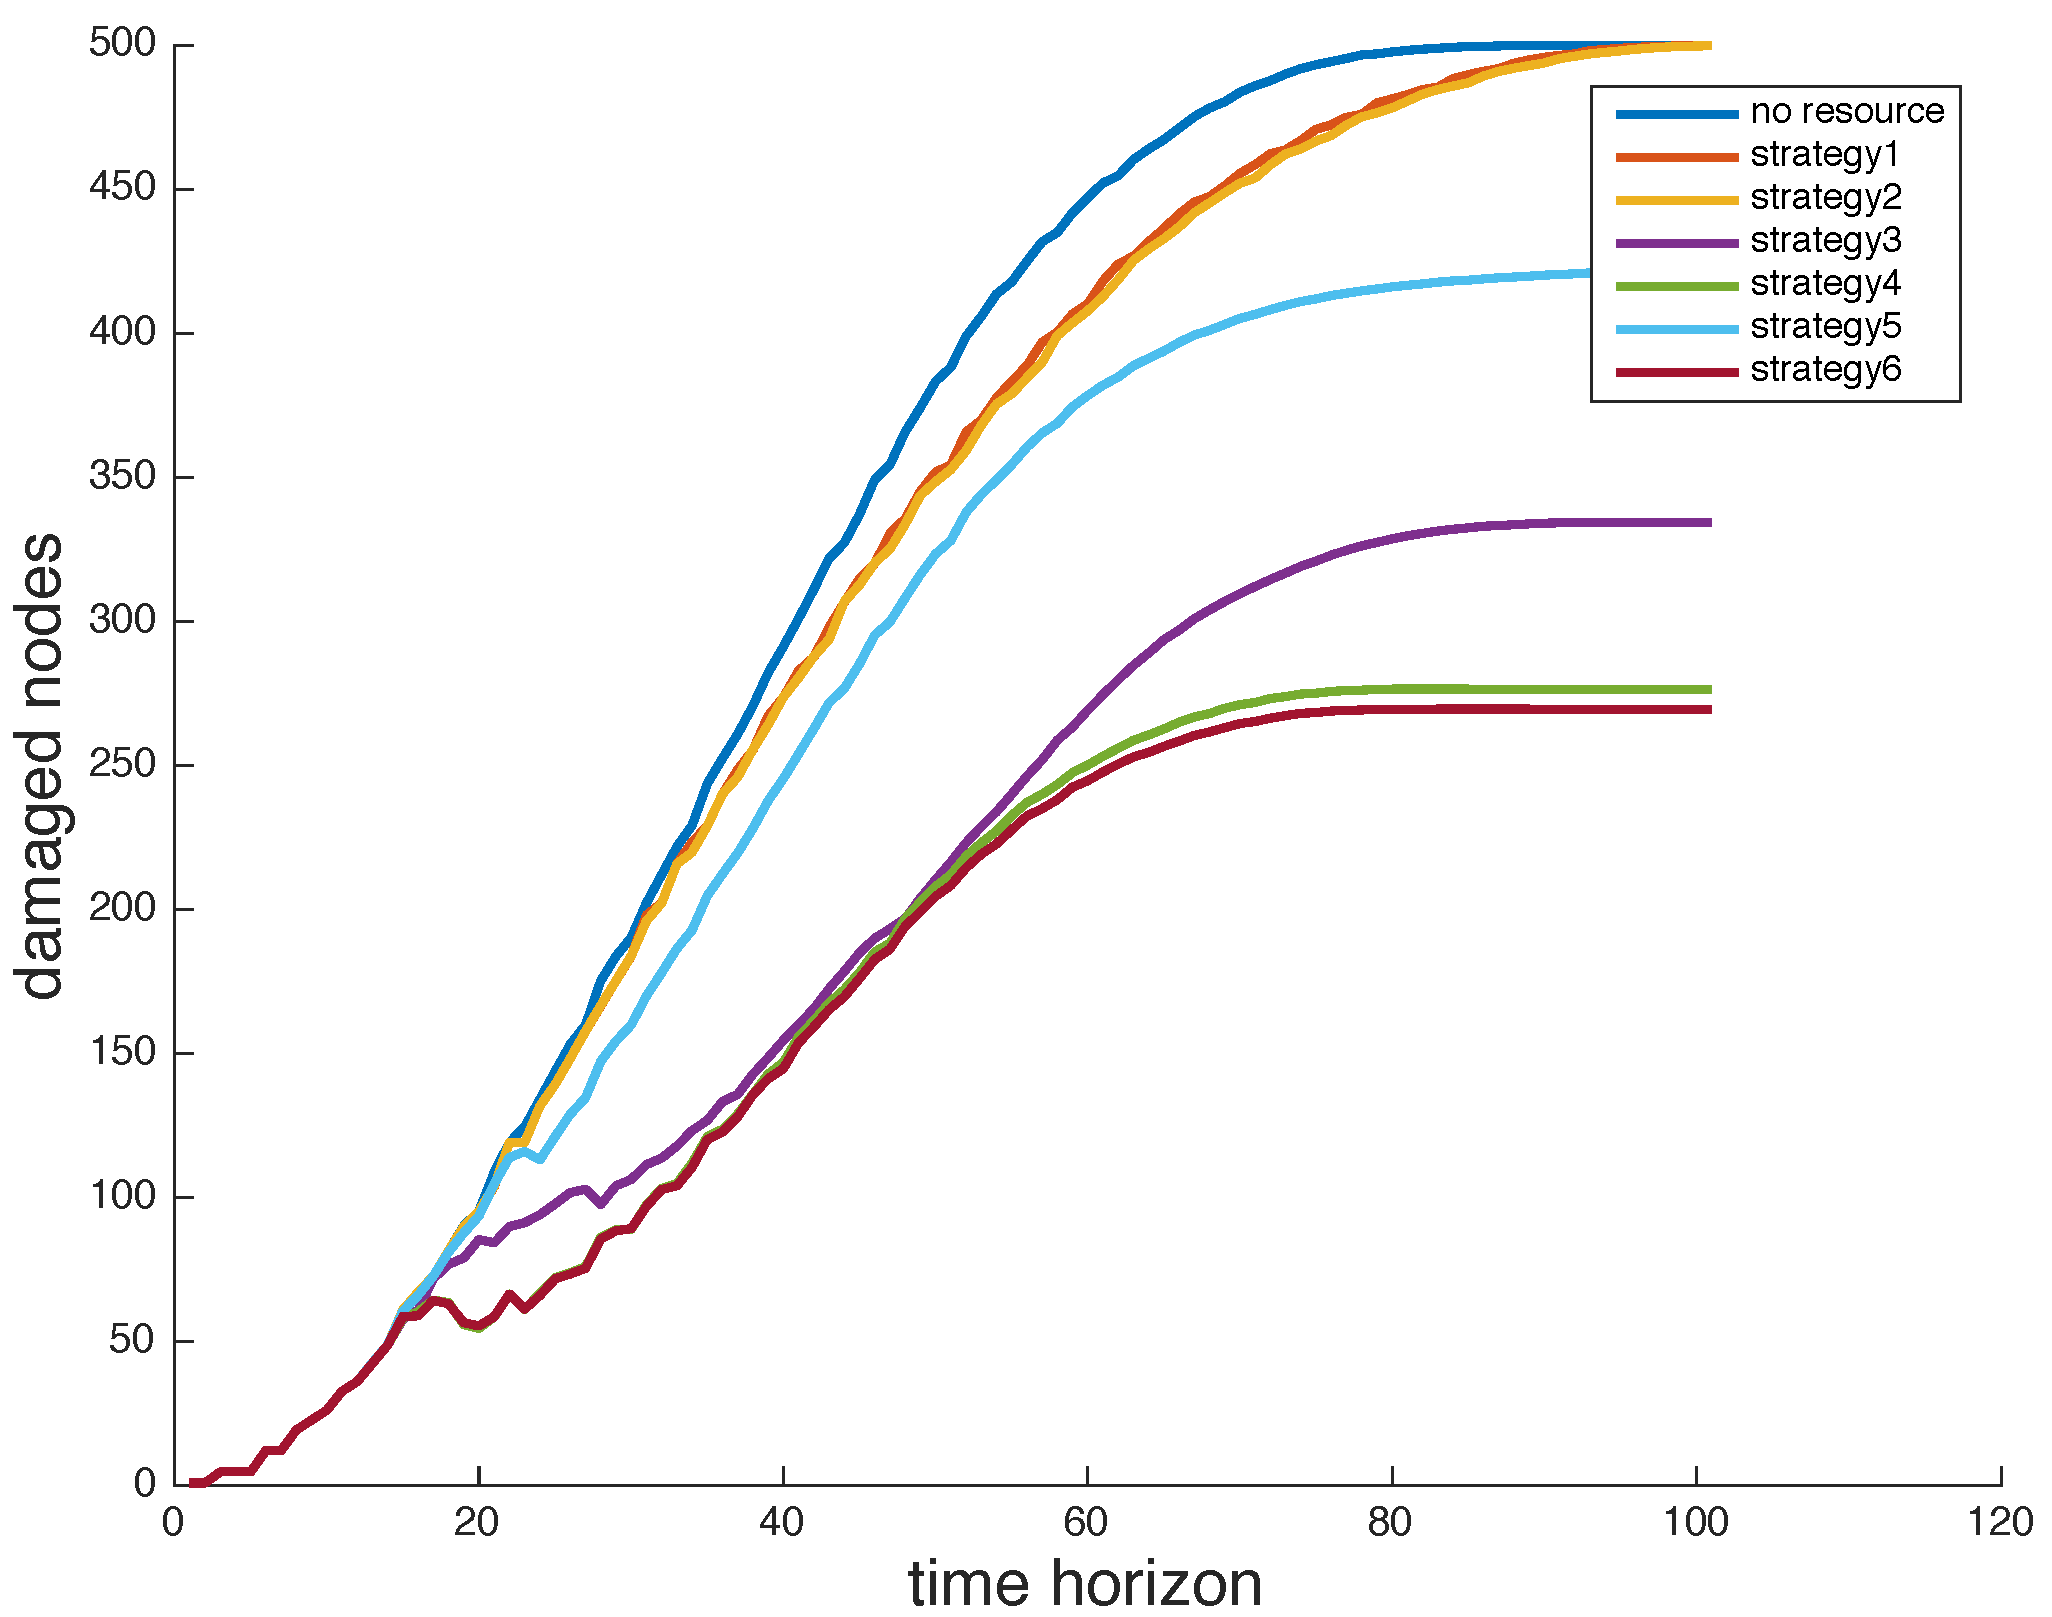
\includegraphics[height=80mm]{../figs/GridNet_original_paper2.pdf}
		\caption{Heuristic strategies on GRID network}
	\end{subfigure}
	~
	\begin{subfigure}[t]{0.8\textwidth}
		\centering
		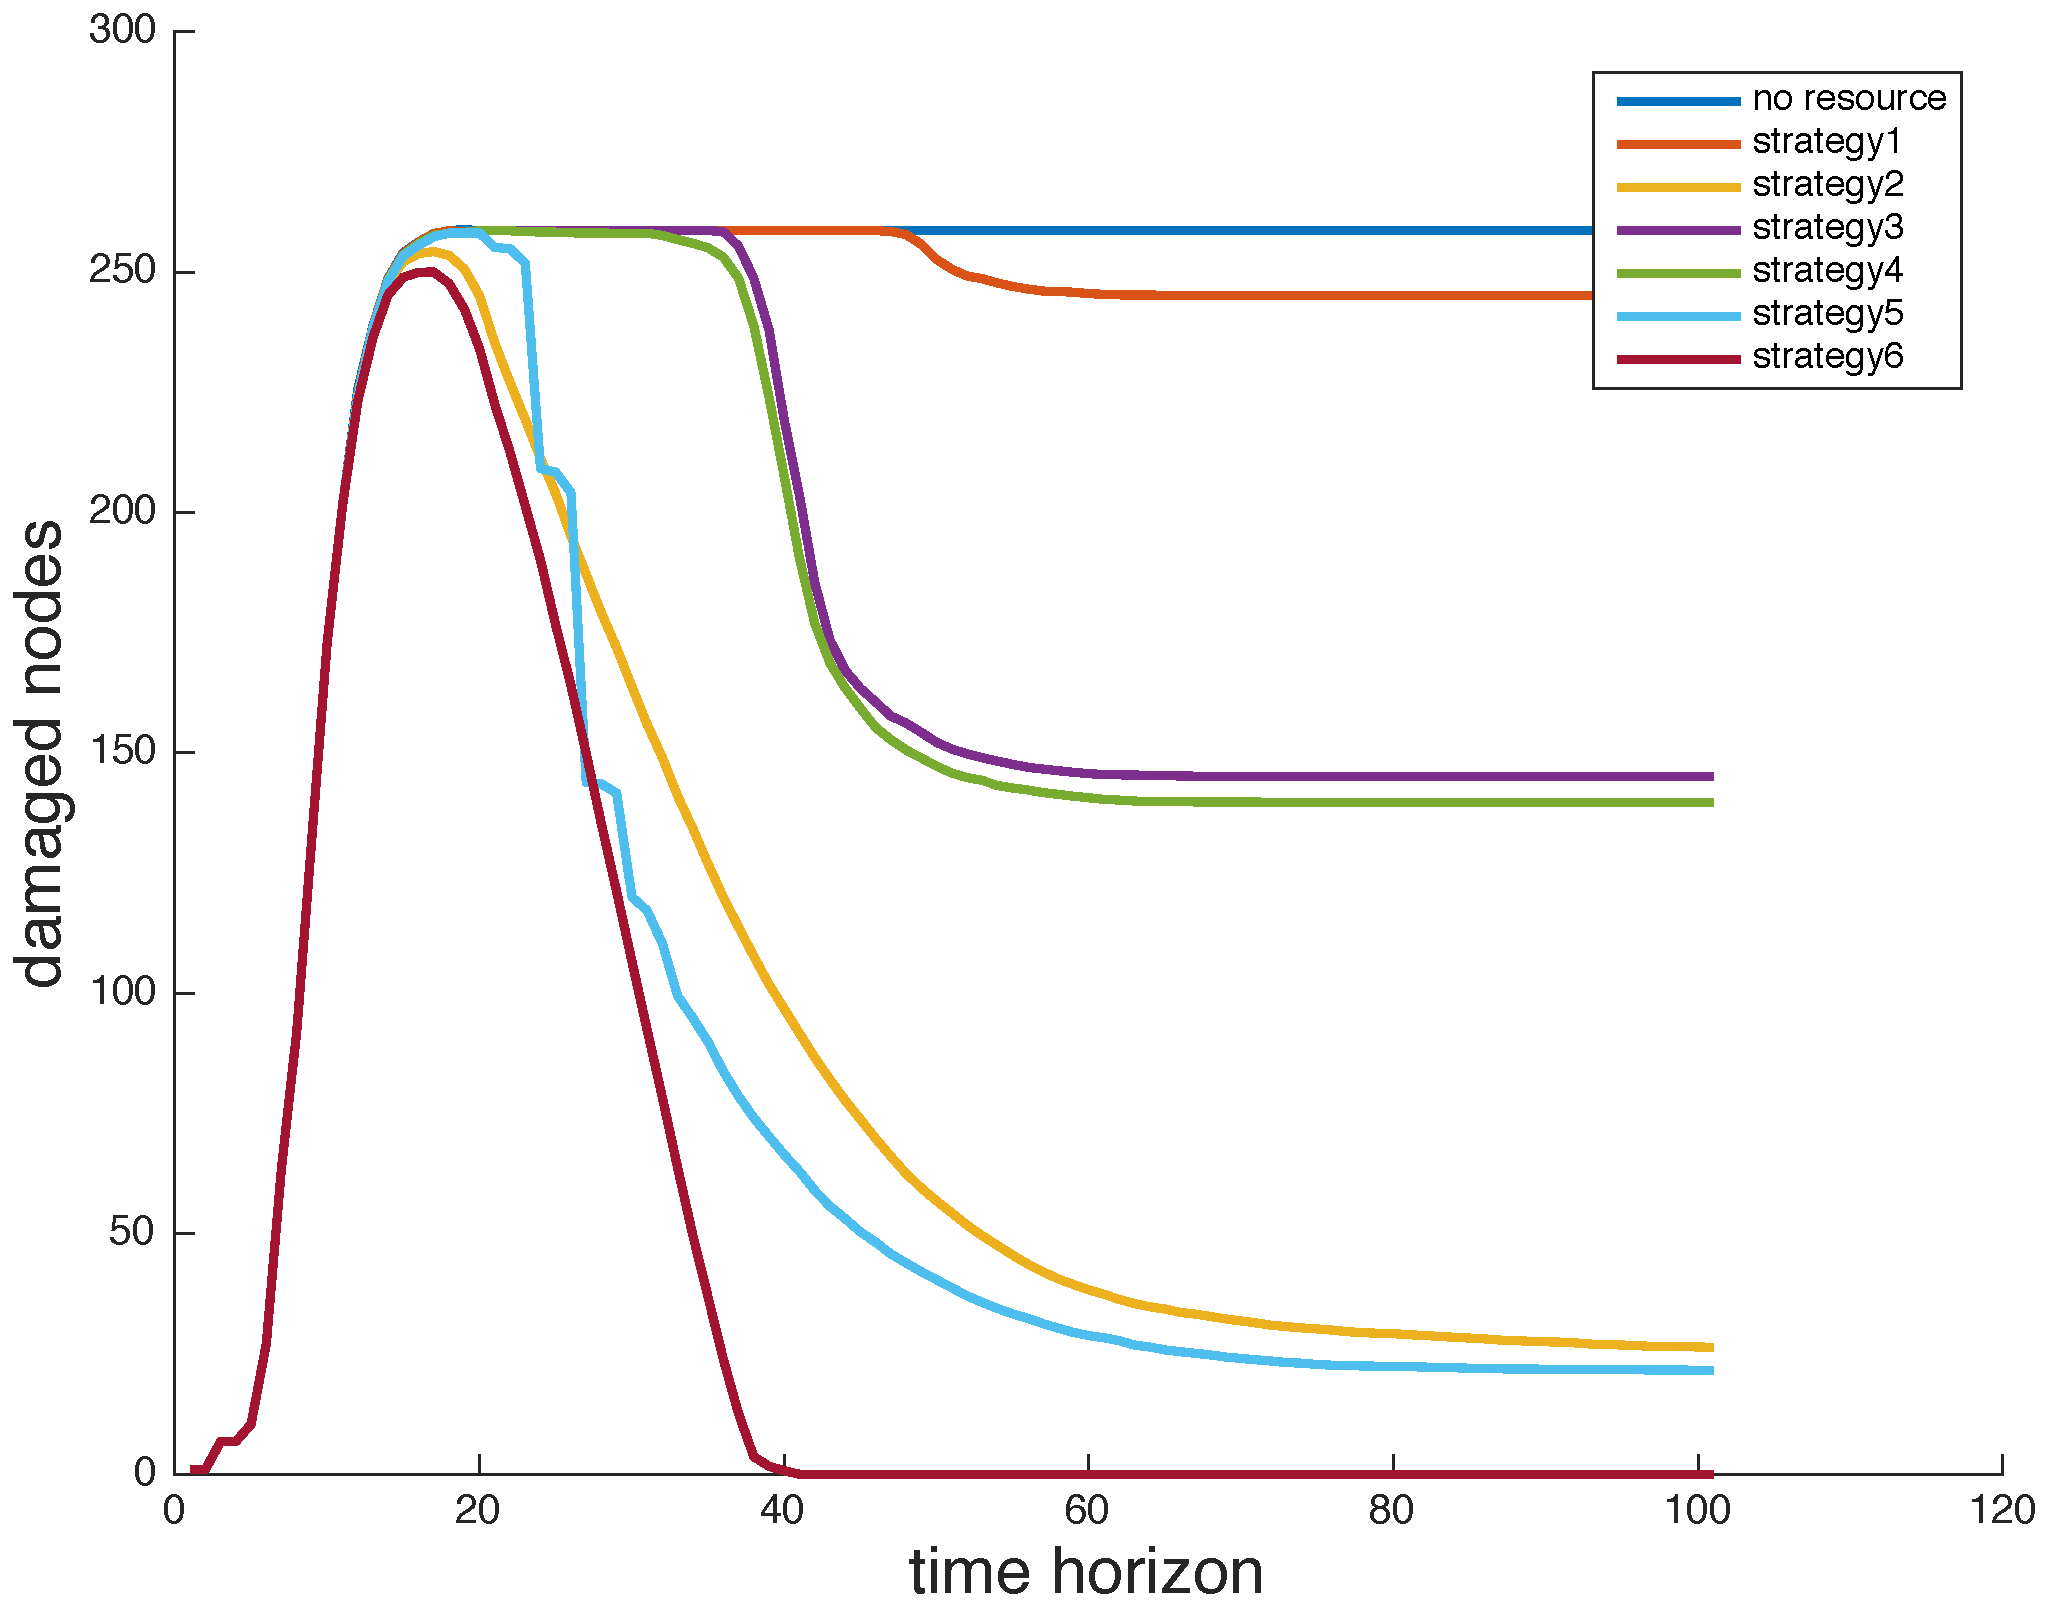
\includegraphics[height=80mm]{../figs/SFNet_original_paper2.pdf}
		\caption{Heuristic strategies on ScaleFree network}
	\end{subfigure}
	\caption{Average number of damaged nodes in (a) grid network and (b) scale-free network, with different heuristic strategis. Total external resources is 1000 and $t_D=8$. The initial damaged node is chosen randomly and these curves is average of 50 experiments.}
	\label{fig:reproduceresult}
\end{figure}
%
we can see that our result (FIG. \ref{fig:reproduceresult}) is almost the same with that in original paper\cite{buzna2007efficient}. This proves the consistency between our model and original model. So, we can further derivate the optimal strategy.

\subsection{The Optimal Strategy}
As said before, we model the disaster spreading as an optimization problem and the solution to this optimization problem corresponds is exactly the optimal strategy to distribute external resources. We have introduced this optimization model in Sec. \ref{sec:adjointmethod} and specified its details in Appendix \ref{sec:appendix1}. Now, we compare the derivated optimal strategy with these six heuristic strategies.


\begin{figure}
	\centering
	\begin{subfigure}[t]{0.8\textwidth}
		\centering
		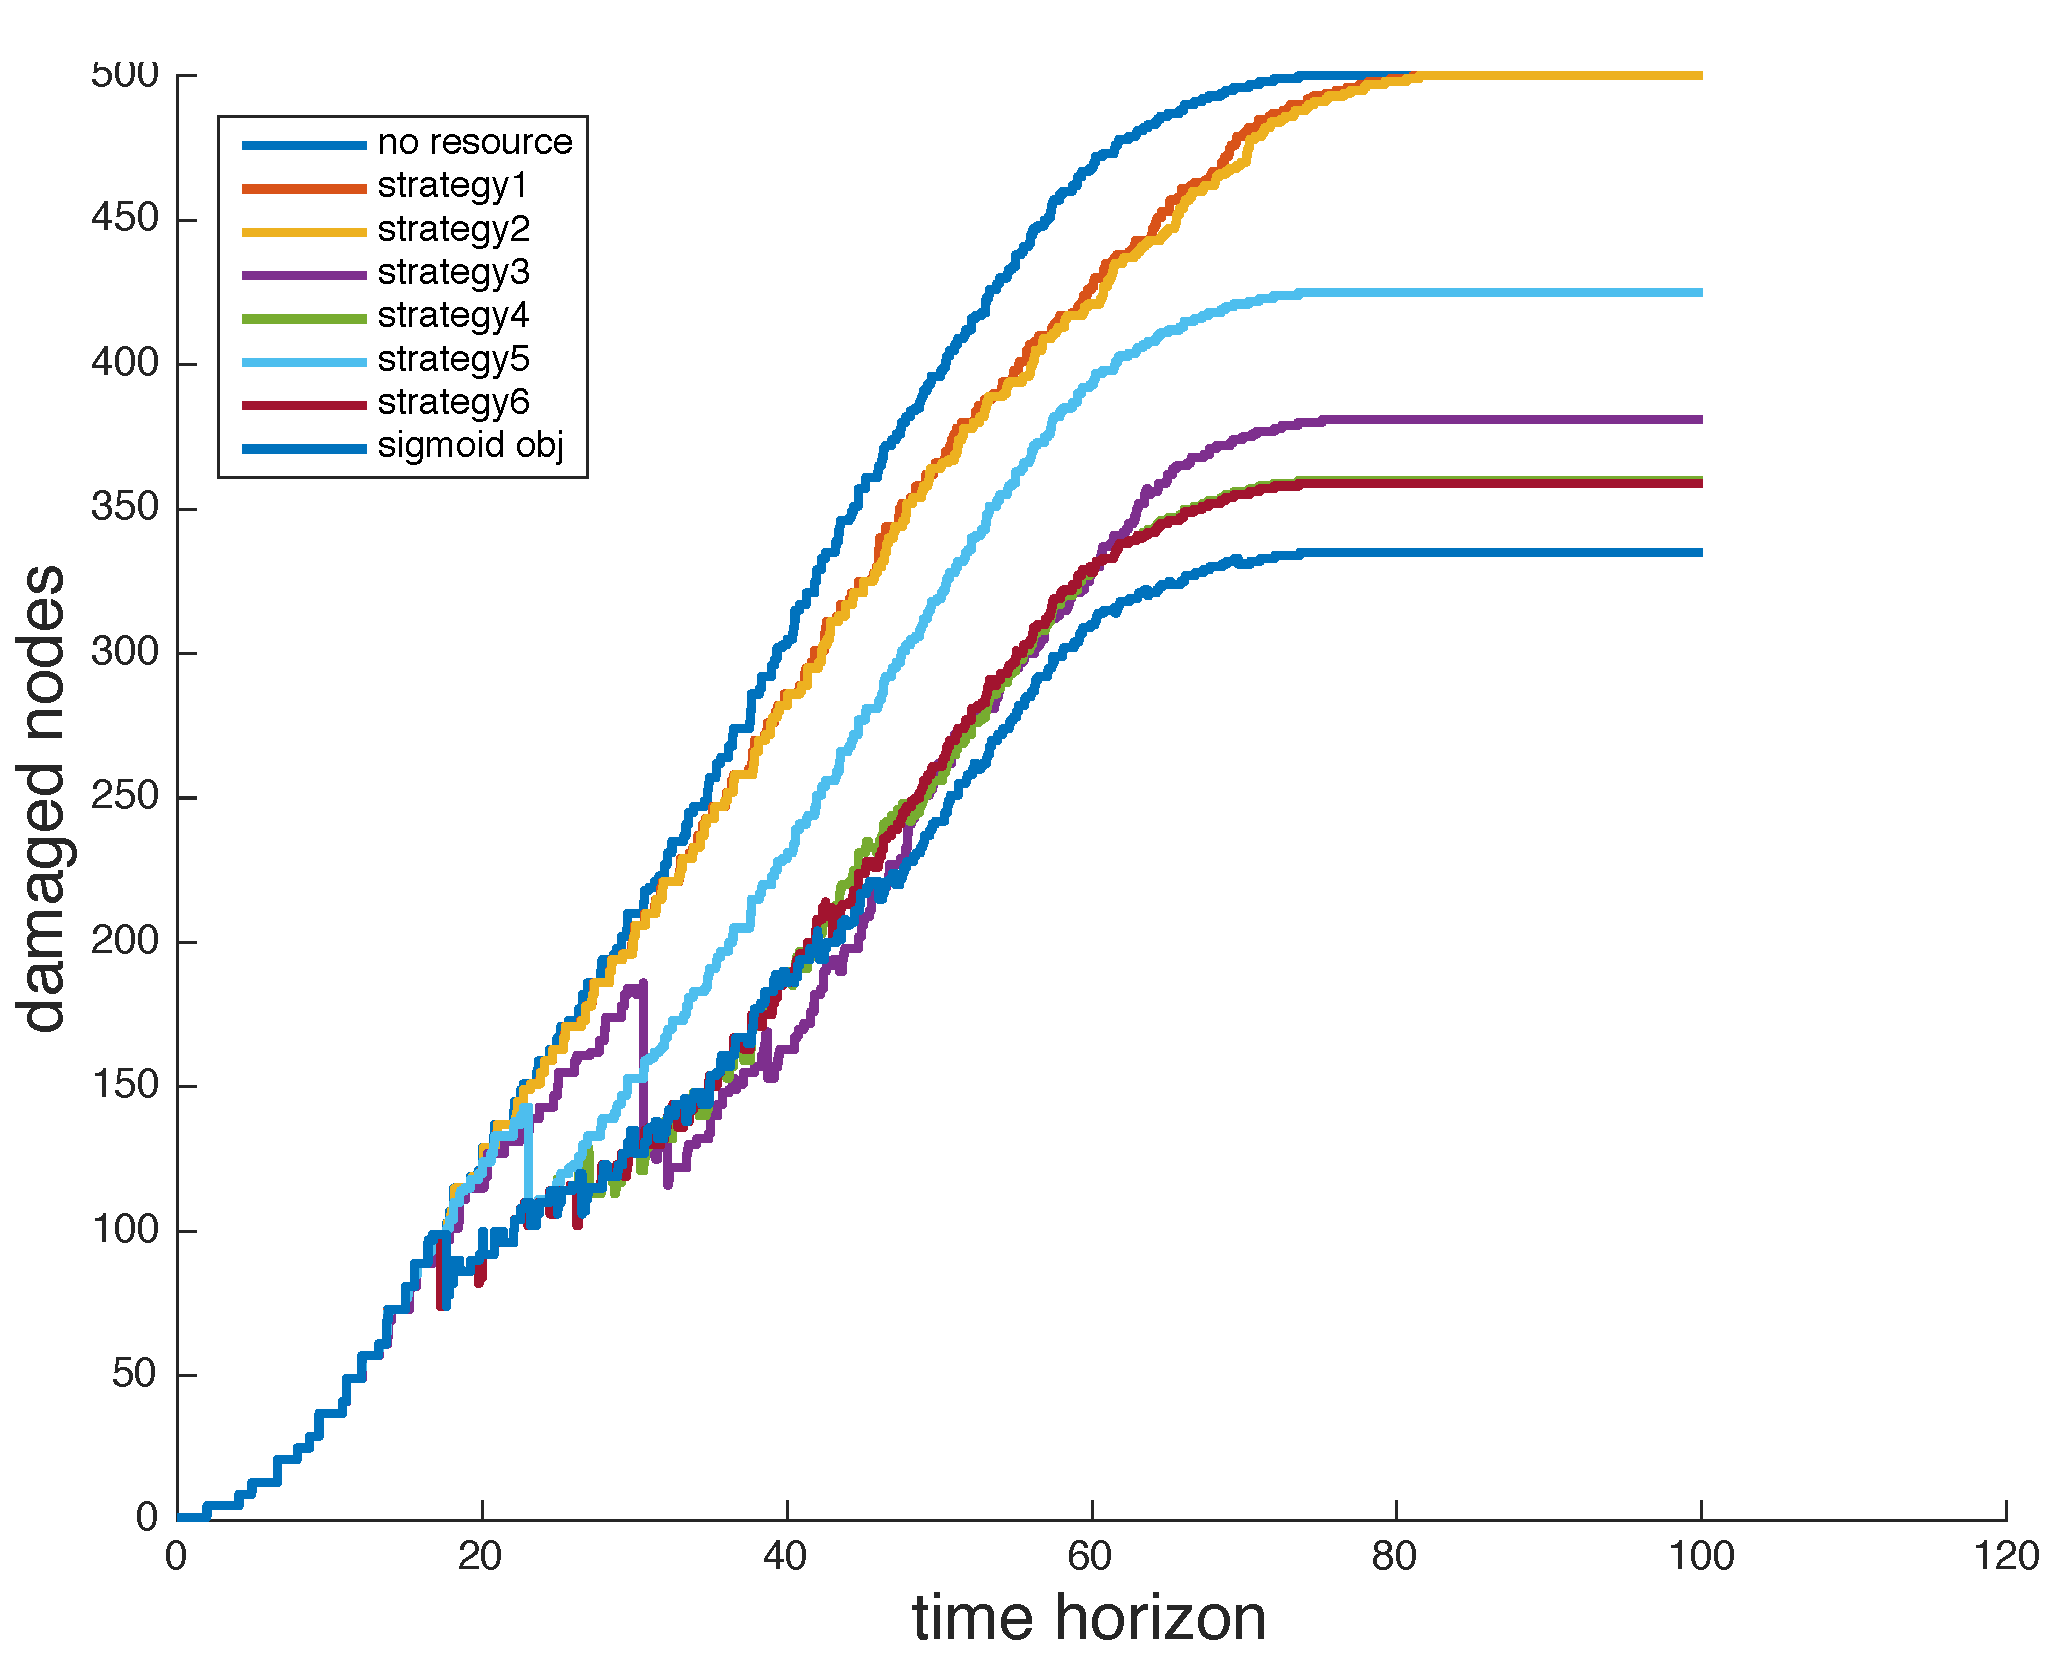
\includegraphics[height=80mm]{../figs/no_linear_approximation/Grid_damaged_small.pdf}
		\caption{Damaged nodes on grid network}
	\end{subfigure}
	~
	\begin{subfigure}[t]{0.8\textwidth}
		\centering
		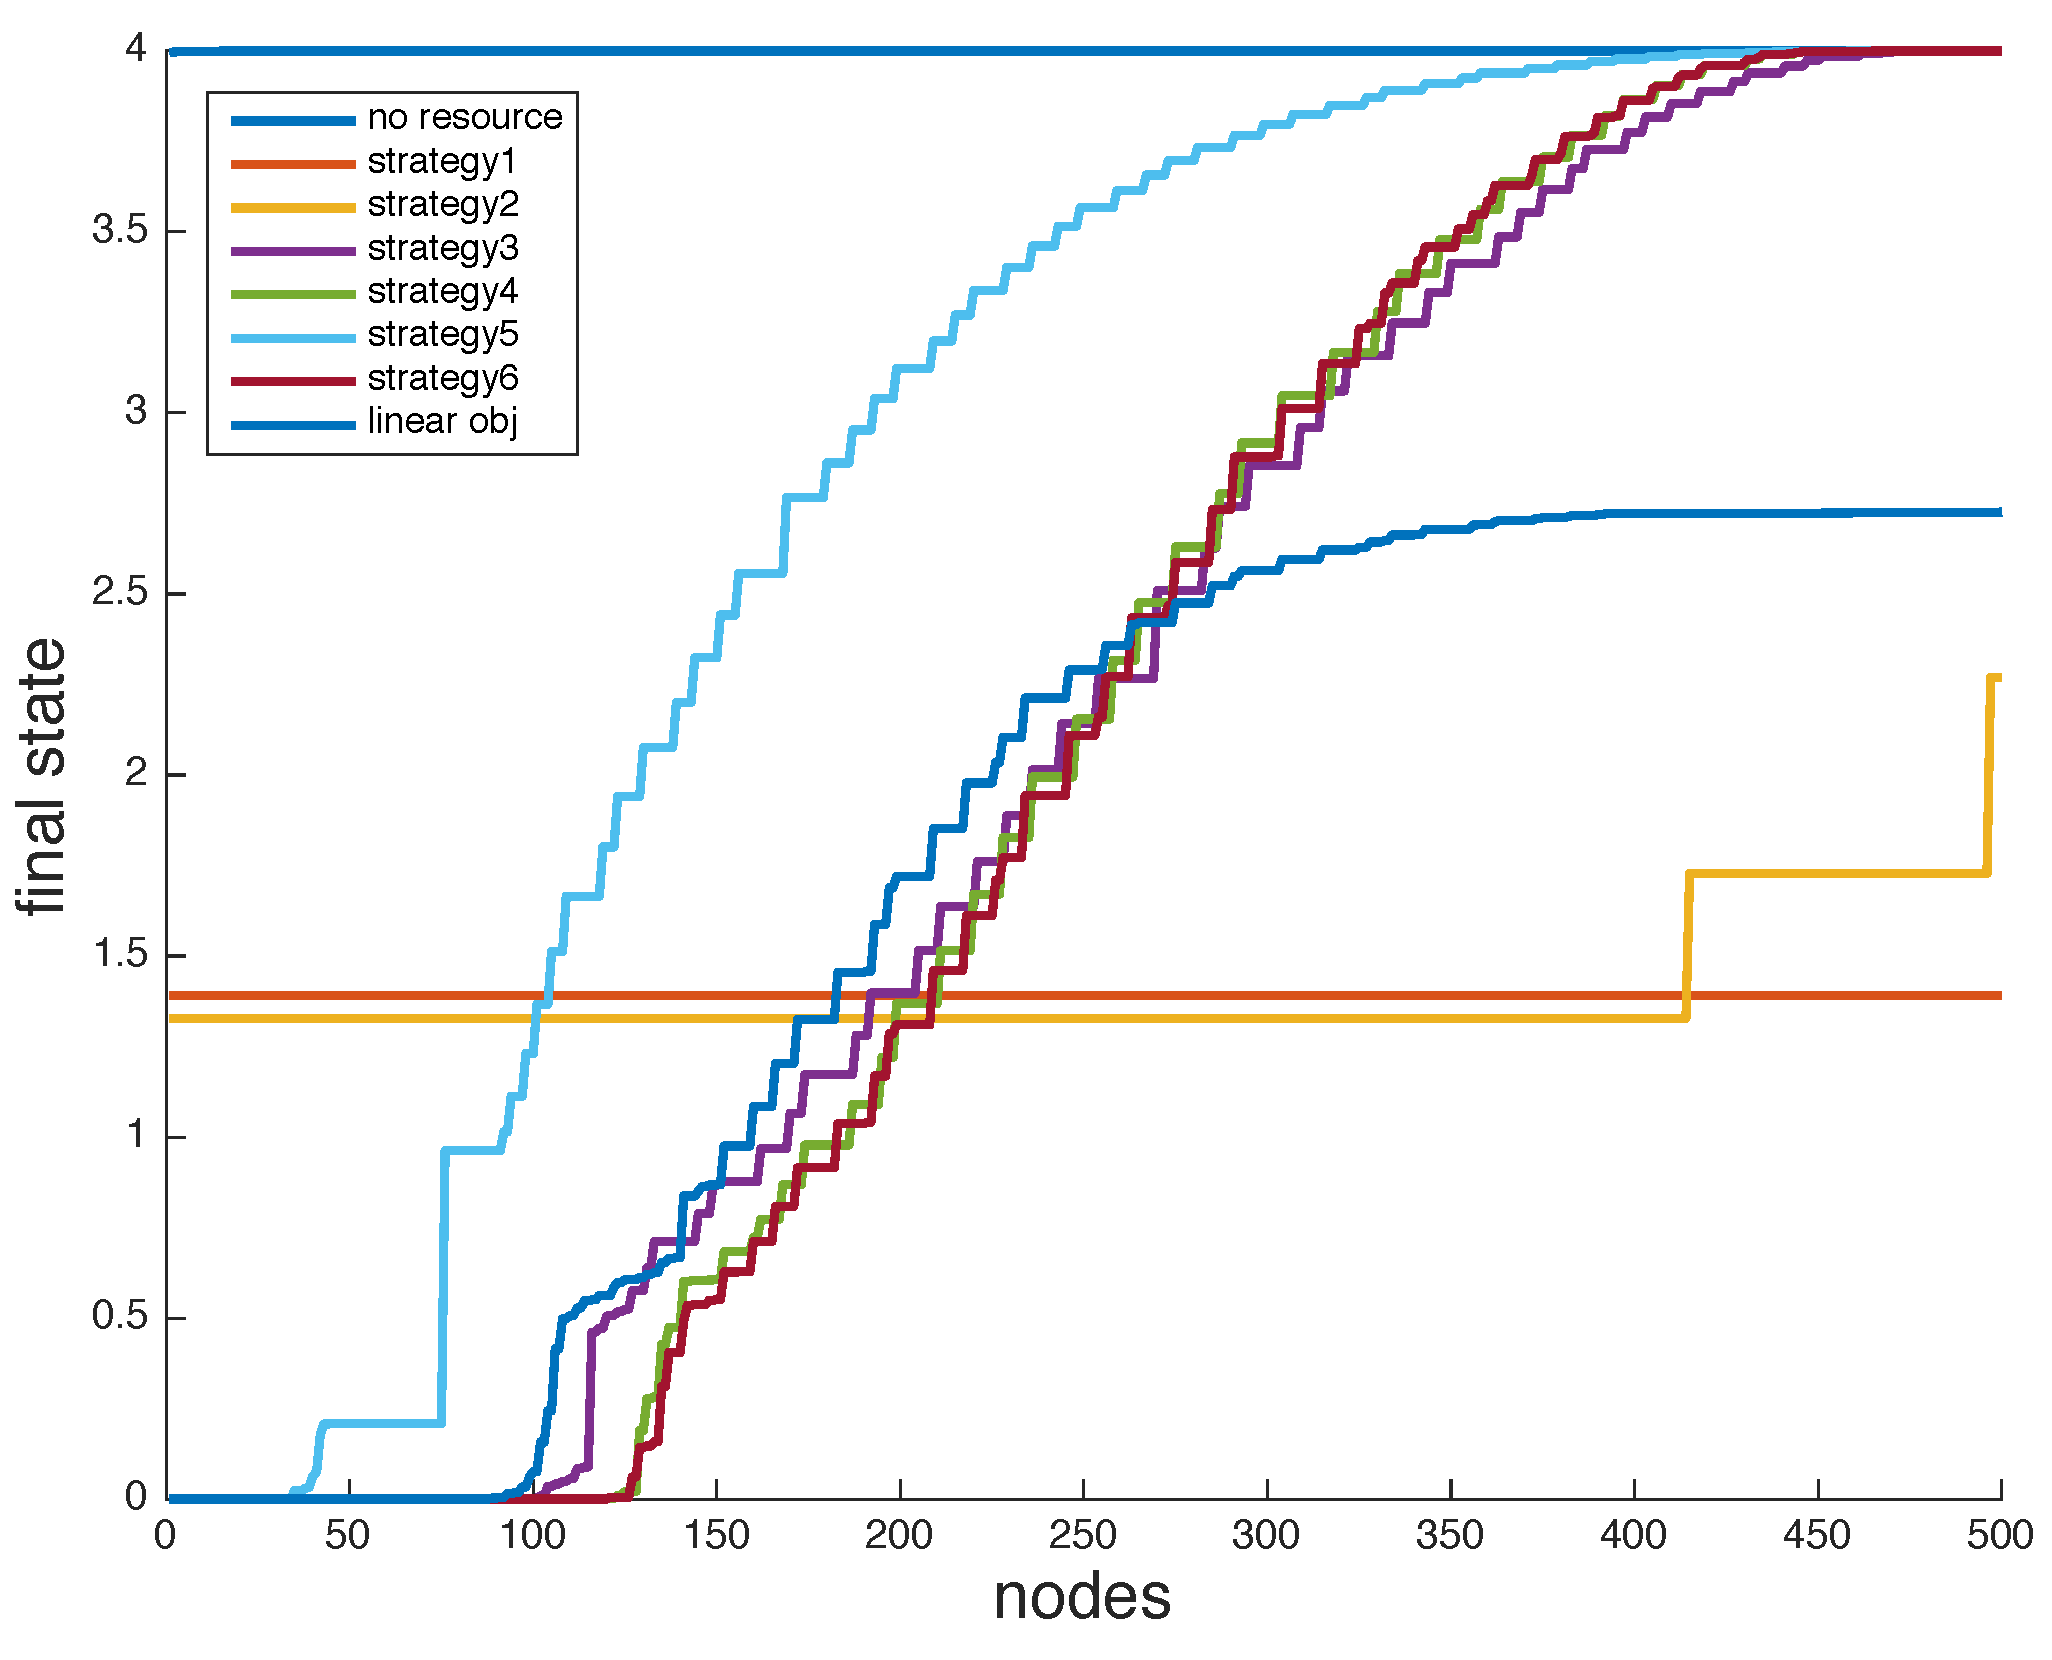
\includegraphics[height=80mm]{../figs/no_linear_approximation/Grid_finalState_small.pdf}
		\caption{Final states on grid network}
	\end{subfigure}
	\caption{(a) Number of damaged nodes and (b) final states on grid network. Total external resources is 1000 and $t_D=8$. The initial damaged node is chosen randomly. The maximal iterations of gradient descent is 100.}
	\label{fig:opt_on_grid}
\end{figure}

We first minimize the number of damaged nodes. A natural objective function for this purpose is 0-1 loss function:

\begin{equation}
	\label{eq:0_1_loss}
	\begin{aligned}
		J &= \sum_i h(x_i) \\
		\text{where } h(\cdot) &= 
		\begin{cases}
			1 & \text{if } x_i \ge \theta_i \\
			0 & \text{otherwise}
		\end{cases}
	\end{aligned}
\end{equation}

However, this objective function is not continuous and cannot be optimized by the adjoint method. So we use again the sigmoid function to approximate this 0-1 loss function:

\begin{equation}	
	\label{eq:sigmoid2}
	\Theta_i(y) = \frac{1-\exp(-\alpha y)}{1+\exp(-\alpha (y-\theta_i))}
\end{equation}

The $\alpha$ parameter in formula \ref{eq:sigmoid2} controls its shape. We find that the sigmoid can approximate the 0-1 loss function very well with $\alpha \leq 20$. So we set $\alpha=20$ and compare the derivated strategy with other six heuristic strategies. Fig. \ref{fig:opt_on_grid} shows that this derivated optimal strategy do decrease the number of damaged nodes.

\begin{figure}
	\label{eq:sigmoid_alpba}
	\centering
	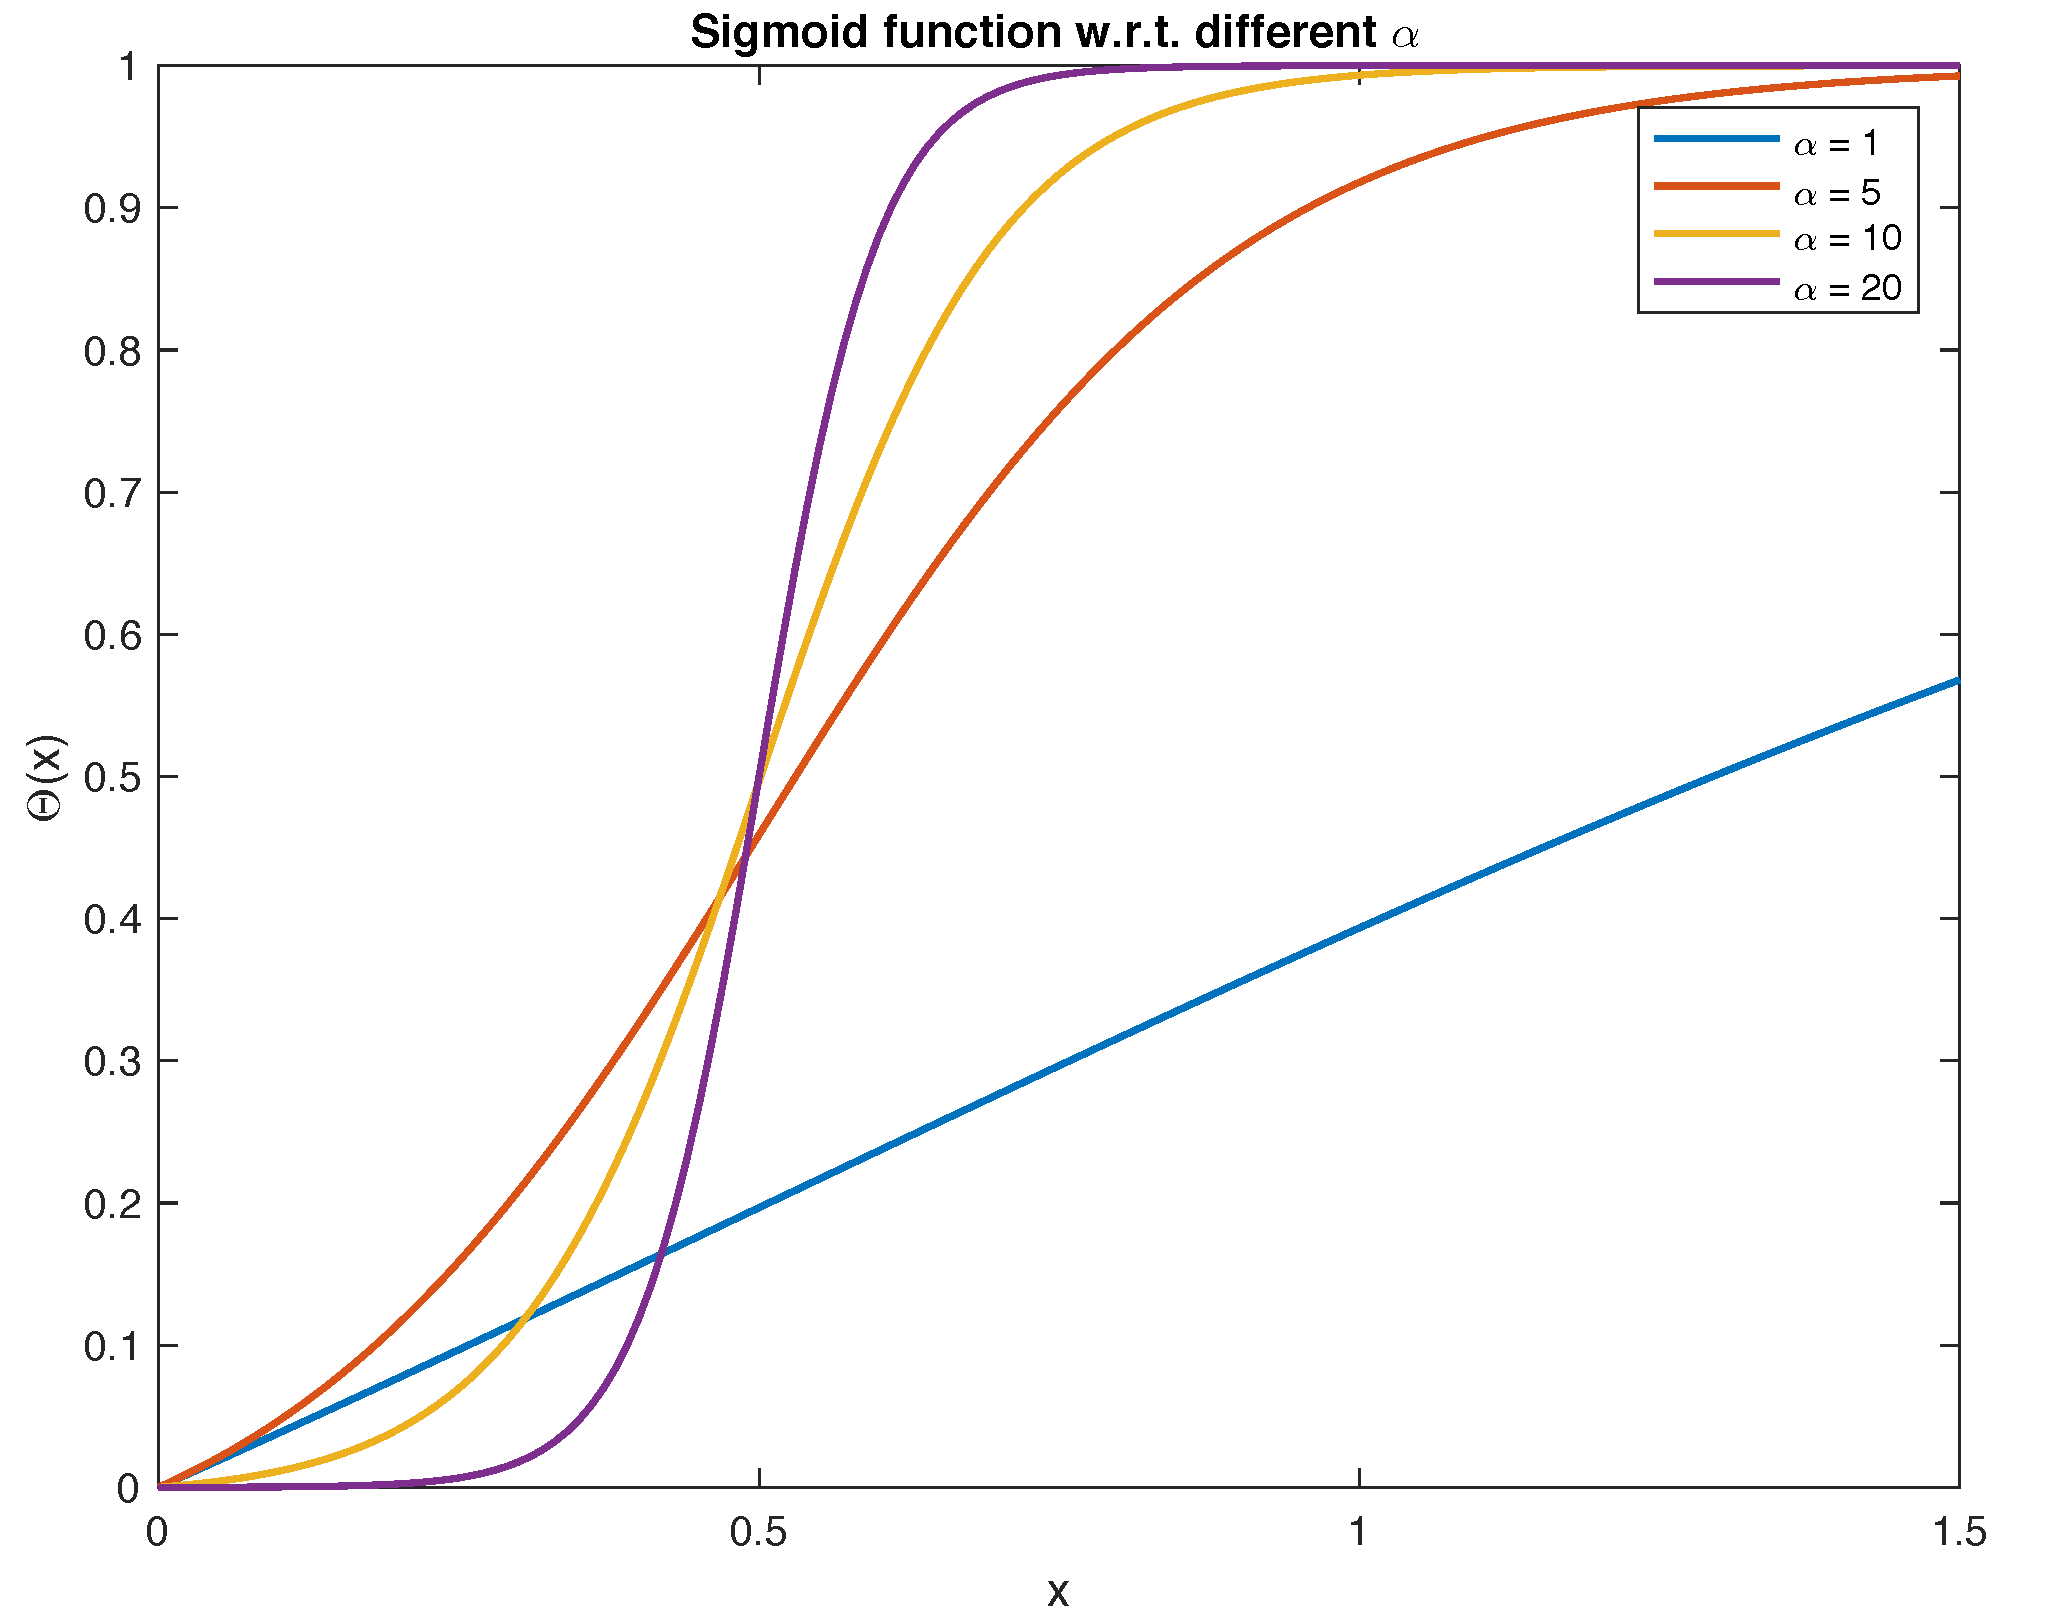
\includegraphics[height=60mm]{../figs/sigmoid_small.pdf}
\end{figure}

However in some cases, we care about the states of all nodes and we do not want to lose control on some nodes. And it is not insufficient to use the number of damaged nodes as criterion to evaluate strategies, since some strategy may abandon those nodes which are severely damaged. Based on such consideration, we proposed the other objective function:

\begin{equation}
\label{eq:obj2}
	J = \frac{1}{n} \sum_i x_i
\end{equation}

Eq. \ref{eq:obj2} aims at optimizing the average state of all nodes. It exclude the situation that some nodes are out of control. FIG. \ref{fig:opt_on_grid} (b) compares the optimal strategy corresponding to this objective function with other heuristic strategies. We can find that the derivated optimal strategy do optimize the states of all nodes.


Besides the grid network, we also perform the same experiments on scale-free network. The result (FIG. \ref{fig:opt_on_sf}) shows that the derivated strategy is again better than other six heuristic strategies.

\begin{figure}	
	\centering
	\begin{subfigure}[t]{0.8\textwidth}
		\centering
		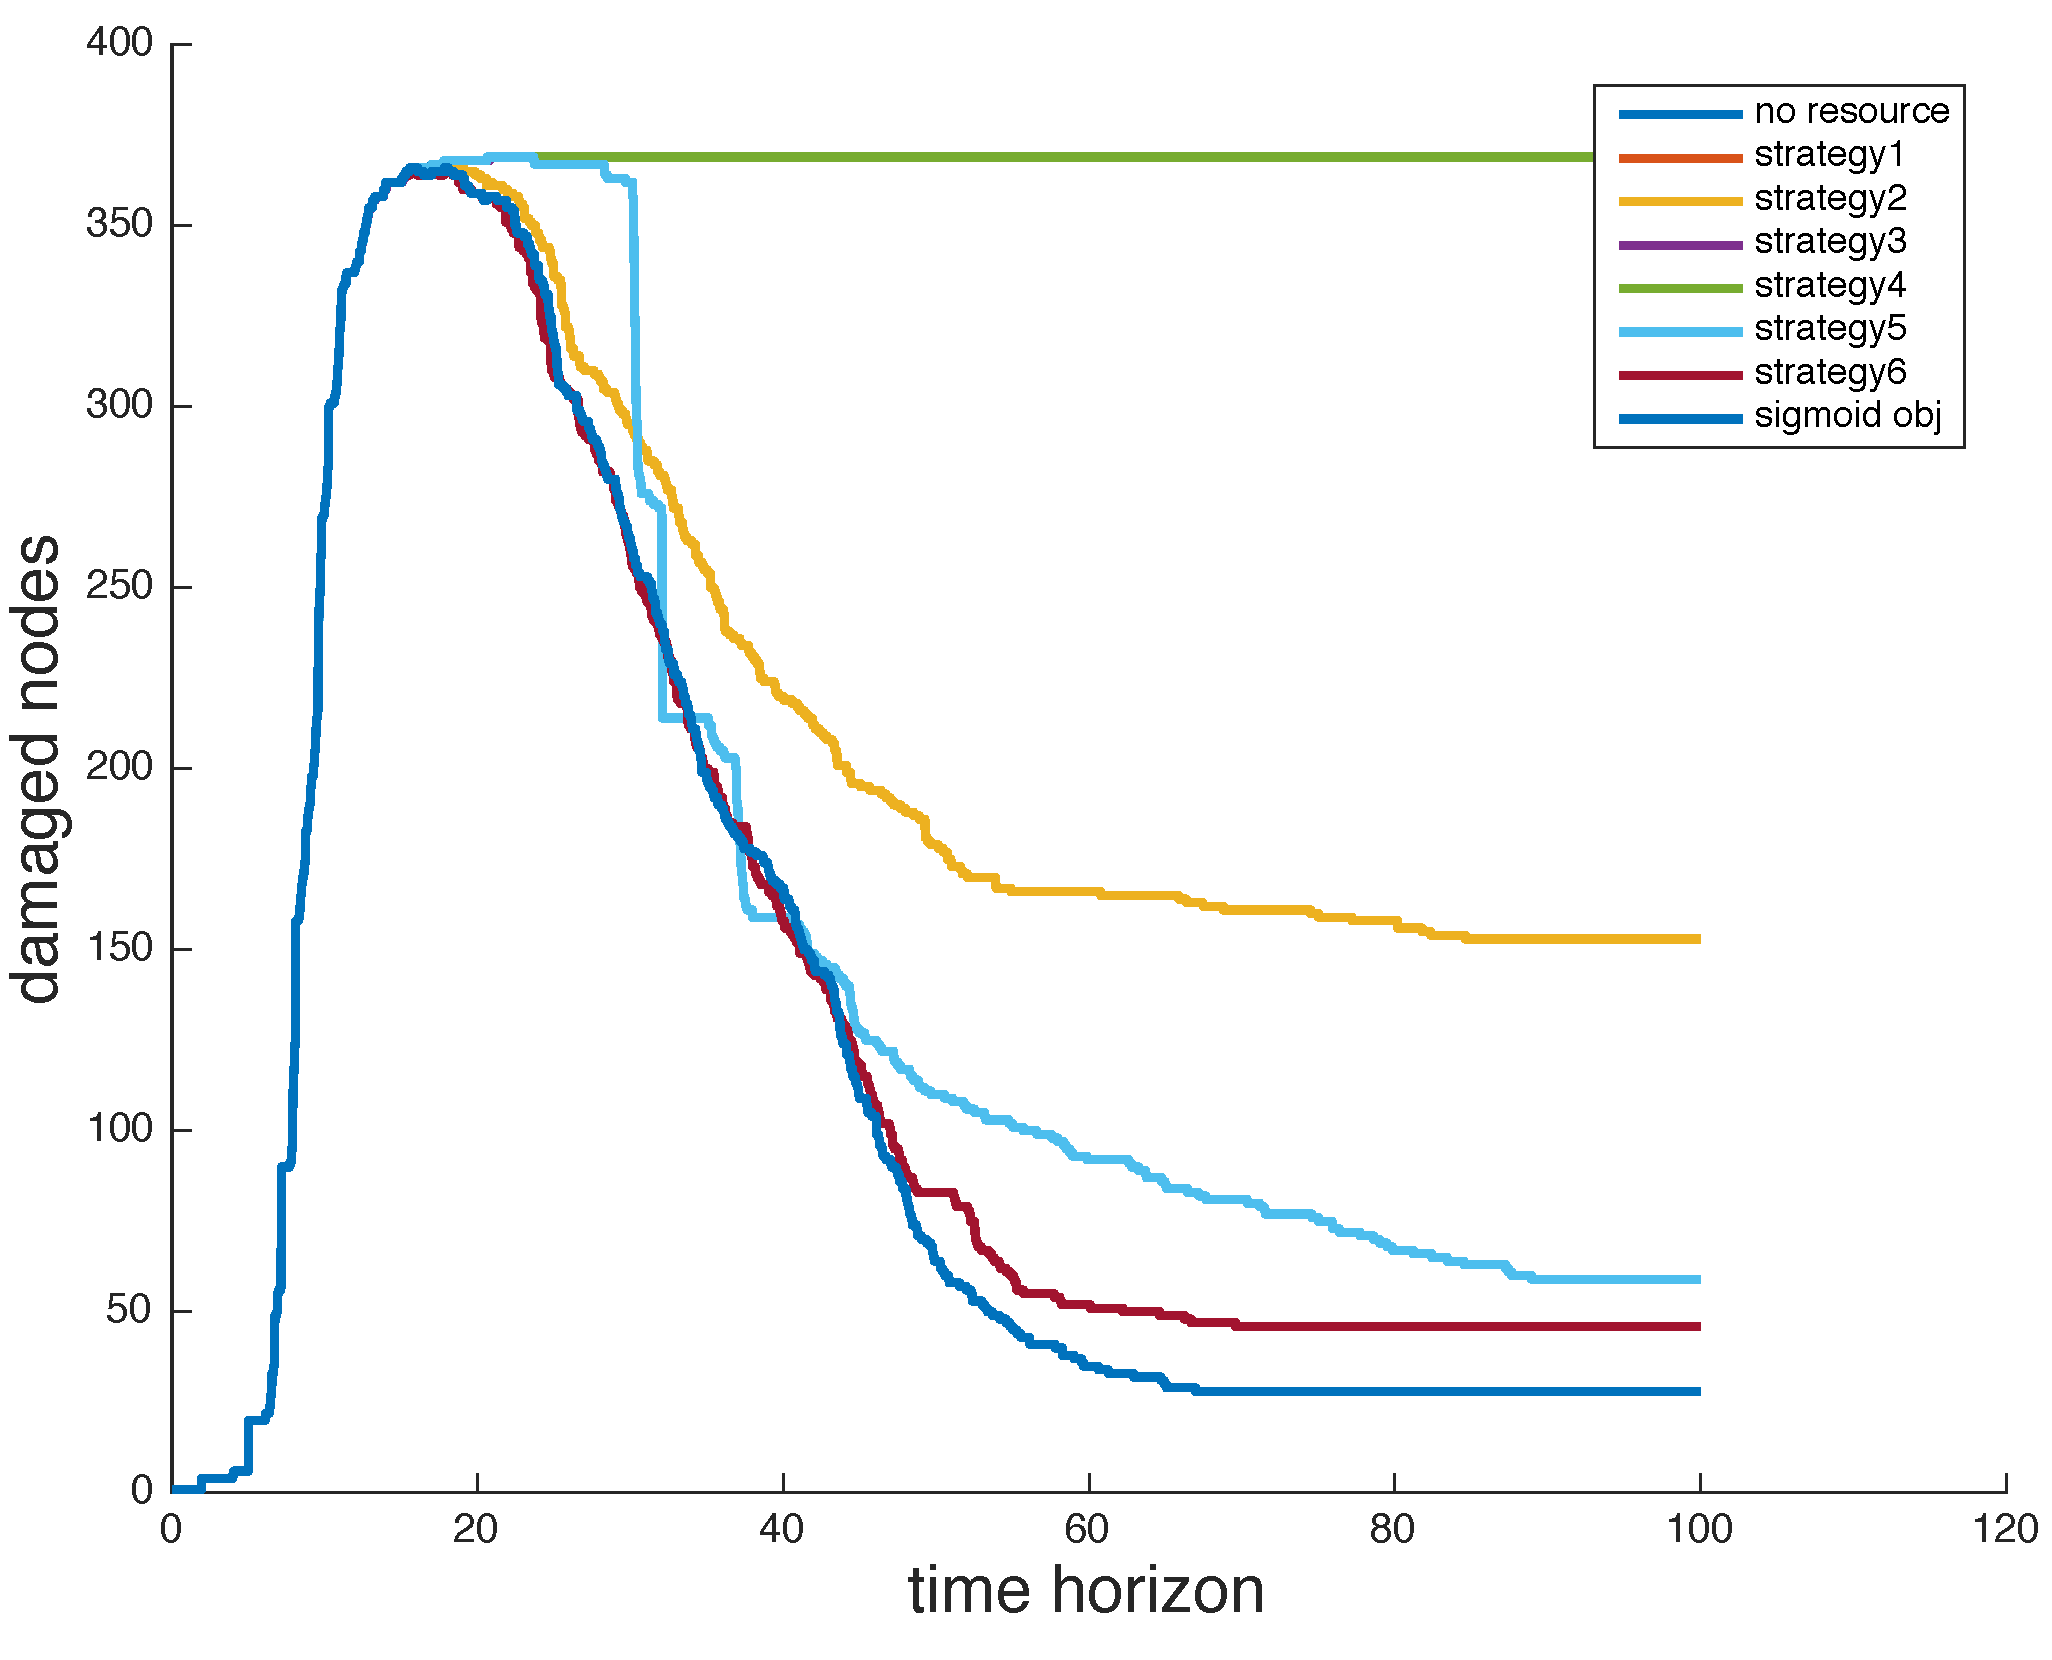
\includegraphics[height=80mm]{../figs/no_linear_approximation/SF_damaged_small.pdf}
		\caption{Damaged nodes on scale-free network}
	\end{subfigure}
	~
	\begin{subfigure}[t]{0.8\textwidth}
		\centering
		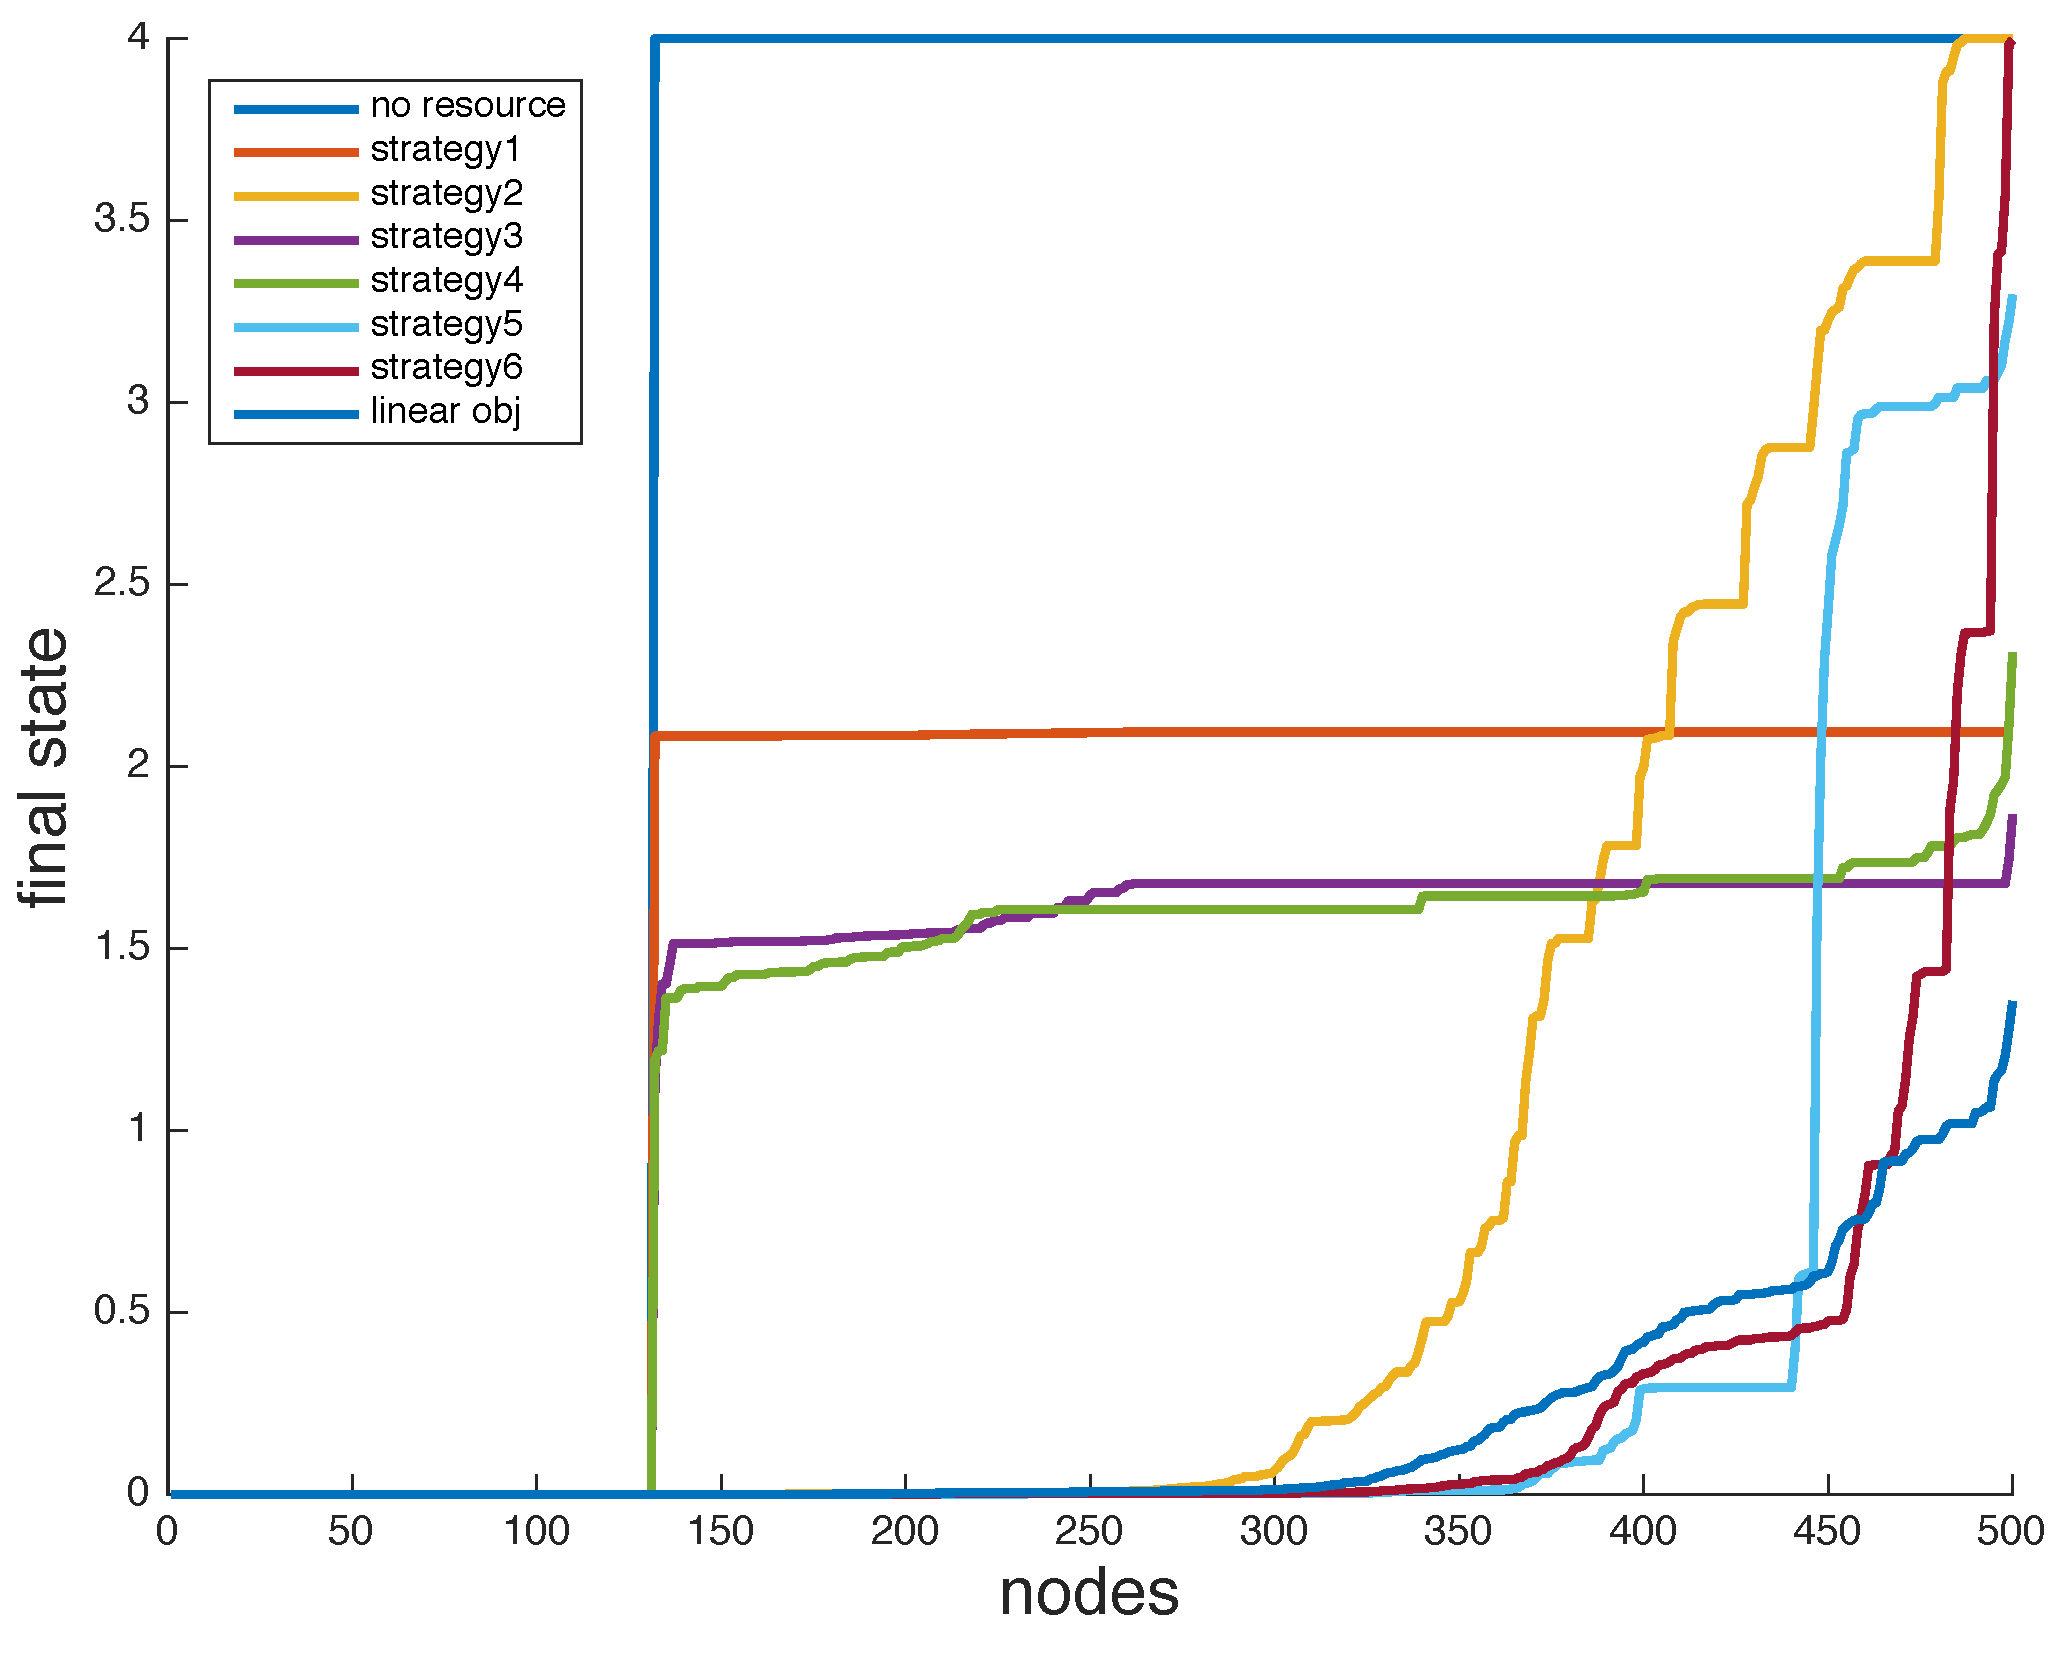
\includegraphics[height=80mm]{../figs/no_linear_approximation/SF_finalState_small.pdf}
		\caption{Final states on scale-free network}
	\end{subfigure}
	\caption{(a) Number of damaged nodes and (b) final states on grid network. Parameter setting is the same with that in grid network except for total external resources, i.e. $t_D=8$ and maximal iterations of gradient descent is 100. Because \textbf{S6} has achieve best result with 1000 external resources, in order to discriminate these strategies we decrease external resources to 600.}
	\label{fig:opt_on_sf}
\end{figure}



